%---------------------------------------------------------------------
% Course 	: Introduction To web sciences
% Professor : Dr.Nelson
% Name   	: Msnoj Chandra Kompalli
% Assignment: 6
%---------------------------------------------------------------------
\documentclass[12pt]{article}
%--------------------------------------------------------------------
% packages required
%--------------------------------------------------------------------
\usepackage{graphicx}
\usepackage{listings}
\usepackage{hyperref}
\usepackage{caption}
\usepackage{color}
\usepackage{pdfpages}
\graphicspath{ {images/} }
%--------------------------------------------------------------------
% Start Margins
%--------------------------------------------------------------------
\addtolength{\oddsidemargin}{-.875in}
\addtolength{\evensidemargin}{-.875in}
\addtolength{\textwidth}{1.75in}
\addtolength{\topmargin}{-.885in}
\addtolength{\textheight}{1.95in}
%-------------------------------------------------------------------
% End Margins
%--------------------------------------------------------------------
\definecolor{codegreen}{rgb}{0,0.6,0}
\definecolor{codegray}{rgb}{0.5,0.5,0.5}
\definecolor{codepurple}{rgb}{0.58,0,0.82}
\definecolor{backcolour}{rgb}{0.95,0.95,0.92}
 
\lstdefinestyle{mystyle}{
    backgroundcolor=\color{backcolour},   
    commentstyle=\color{codegreen},
    keywordstyle=\color{magenta},
    numberstyle=\tiny\color{codegray},
    stringstyle=\color{codepurple},
    basicstyle=\footnotesize,
    breakatwhitespace=false,         
    breaklines=true,                 
    captionpos=b,                    
    keepspaces=true,                 
    numbers=left,                    
    numbersep=5pt,                  
    showspaces=false,                
    showstringspaces=false,
    showtabs=false,                  
    tabsize=2
}
 
\lstset{style=mystyle}

\begin{document}

\begin{titlepage}
\title{INTRODUCTION TO WEB SCIENCES:\\*Assignment 6}
\author{Manoj Chandra Kompalli}
\date{17 March 2016}
\maketitle
\end{titlepage}

\tableofcontents
\newpage

\section{Question 1:  }


\subsection{Approach}
 I had 54 followers to start with. I was really confused how to begin but then I realized that all I needed to do was generate a JSON with two arrays. One with the nodes and other with the edges. Almost all the templates for d3 support this JSON format.\par I could loop through my followers and can get their screen names and id’s and can definitely show that they are connected to me, but the complicated task was showing the connections amongst themselves.\par I decided to use Tweepy library. Tweepy would give me a Boolean value showing if the two people were connected or not. I had to write a function which would only take the names if they had atleast one true value. \par That is, either the follower or followed by attribute is true. My next task was to generate the respective id’s of the source and target screen names. I had then appended the data to my JSON array. 



 \newpage

\subsection{Code Listing}
\subsubsection{conections.py to generate the follower JSON}
\lstinputlisting[breaklines=True,language=Python]{../q1/connections.py}
\newpage


\subsection{Generated JSON file}
\begin{figure}[ht]
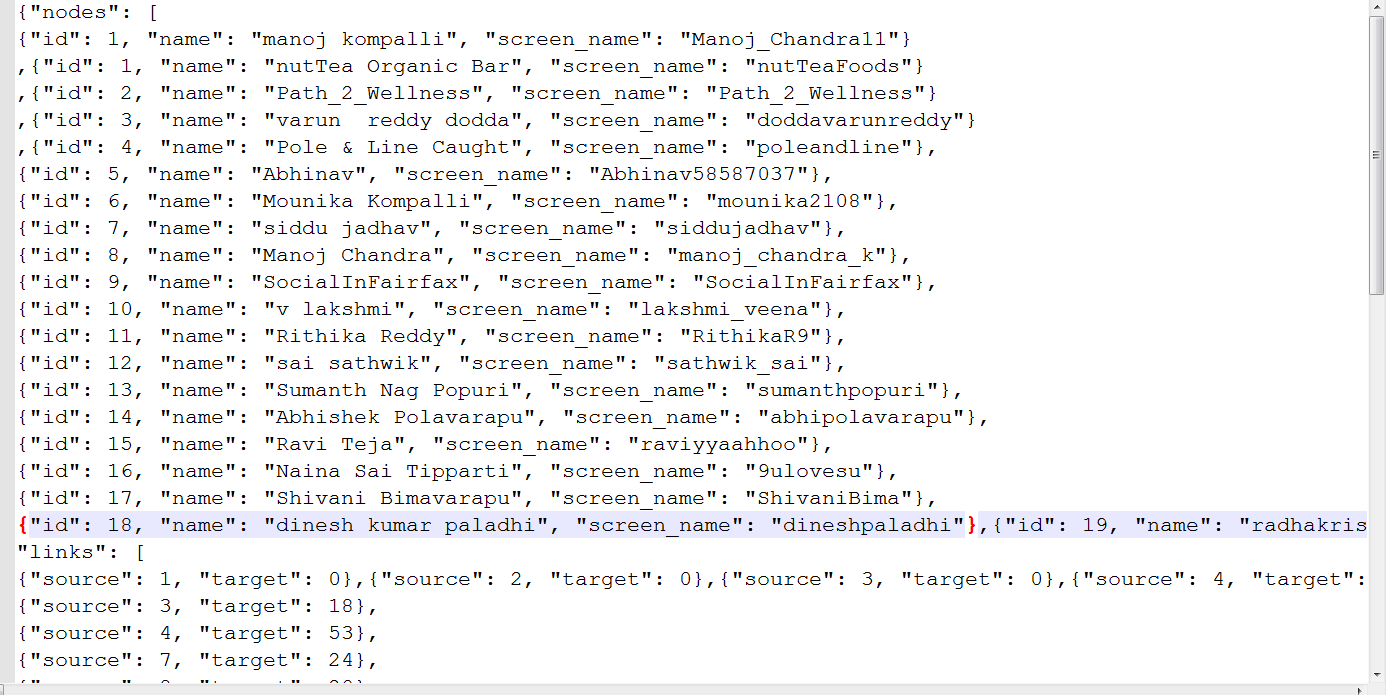
\includegraphics[scale=0.7]{../q1/screenjson.png}
\centering
\caption{JSON array containing the follower data}
\label{fig:JSON array containing the follower data}
\end{figure}

\newpage
\subsection{Graph details}
Here I used an avatar of a cat to show all of my followers. The directed graph has arrows directed from source to target. Example is if  Yeshwanth follows Manoj, the edge is directed from Yeshwanth to Manoj.


\subsection{Force directed graph of twitter followers }
\begin{figure}[ht]
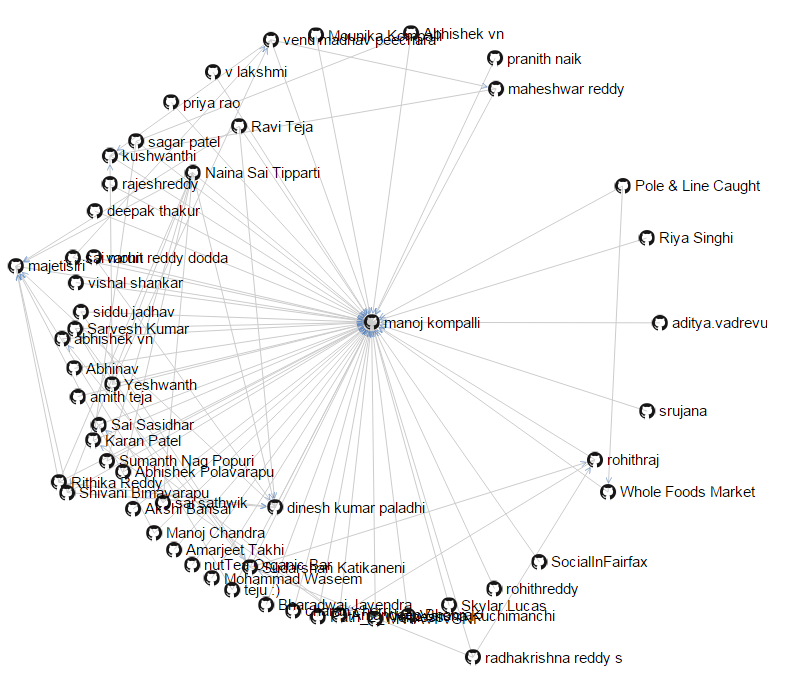
\includegraphics[scale=0.7]{../q1/gr1.png}
\centering
\caption{Twitter followers data of manoj kompalli}
\label{Removed edges}
\end{figure}
\subsection{URI of graph listed in gist}
\url{http://bl.ocks.org/manojchandrak/raw/5794f396fca3ab0dc5b7/}

\newpage
\section{Question 2: }

\subsection{Approach}
 Here, I had used the same JSON data as the above problem. I stripped off the first name from the name. I used urllib2 to run the genderize url on all the first names. I had generated JSON data which had all firstname along with their genders. I had integrated this data into the node data.  I found some entries as null because they were labelled incorrectly or they don’t belong to a person etc. I had generate the force directed graph from this data.

\subsection{Code Listing}
\subsubsection{parse.py}
\lstinputlisting[breaklines=True,language=Python]{../q2/parse.py}
\newpage
\subsection{Code Listing}
\subsubsection{undirected.html}
\lstinputlisting[breaklines=True,language=Python]{../q2/undirected.html}
\newpage
\subsection{Parsed data}

\subsubsection{JSON response based on first name}
\begin{figure}[ht]
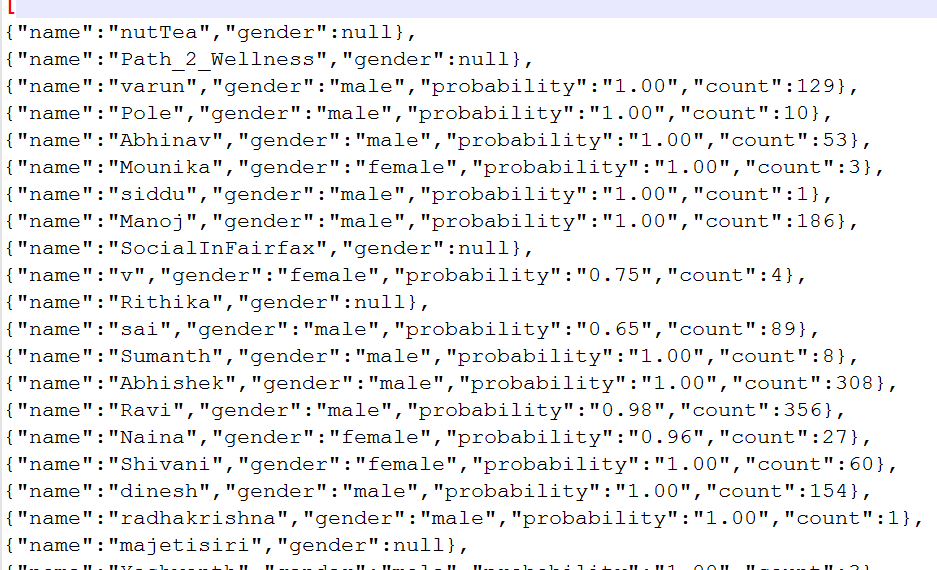
\includegraphics[scale=0.7]{../q2/firstjson.png}
\centering
\caption{Initial graph split into 4 groups}
\label{Initial graph split into 4 groups}
\end{figure}
\newpage

\subsubsection{Follower data with gender details}

 \begin{figure}[ht]
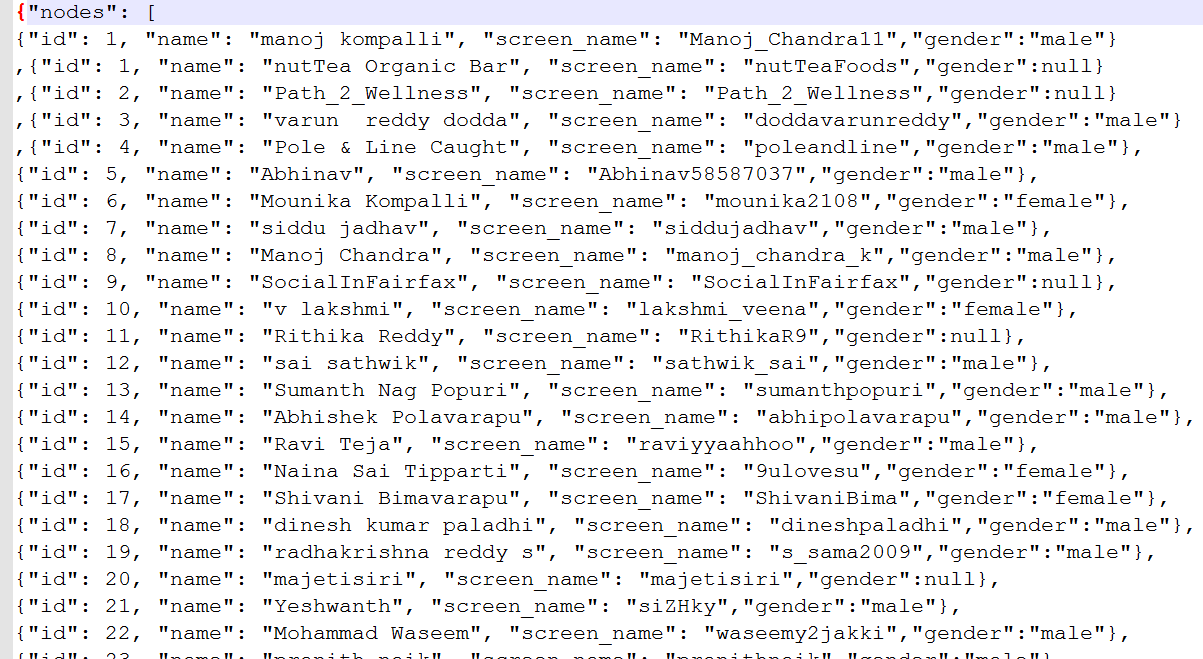
\includegraphics[scale=0.5]{../q2/genderjson.png}
\centering
\caption{Follower data with gender details }
\label{fig:Follower data with gender details}
\end{figure}
\newpage

\subsubsection{Graph details}
 I have figured out that my data had more males which itself is a proof for gender homophily. The blue dots represent the males, the light blue are the nulls and the orange ones represent females. There are only 7 orange nodes and most of them do not have many connections from my followers. This proves gender homophily

\subsubsection{Force directed graph showing gender homophily}
\begin{figure}[ht]
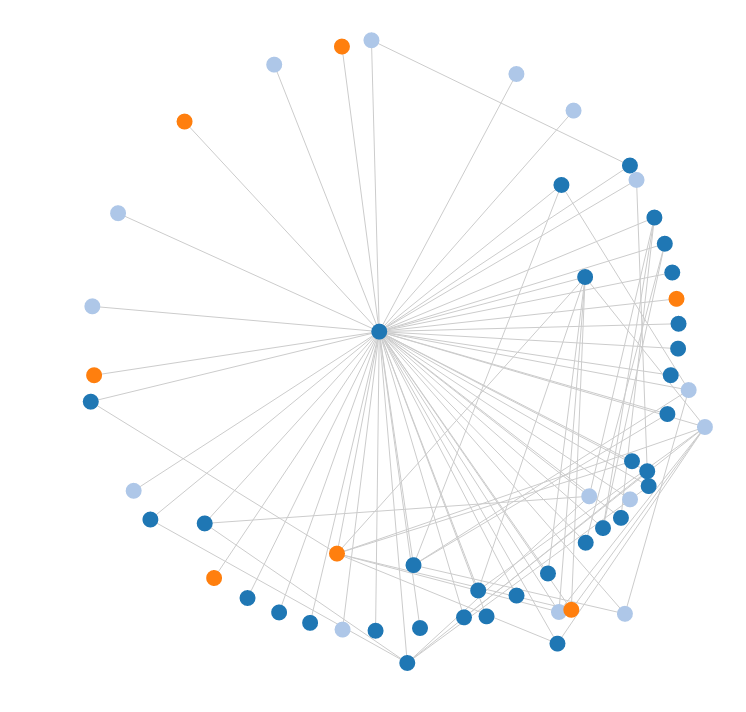
\includegraphics[scale=0.9]{../q2/gr2.png}
\centering
\caption{Force directed graph grouped on gender basis}
\label{Force directed graph showing gender homophily}
\end{figure}
\newpage

\begin{table}

\caption{Table with followers and gender}
\label{Table:q1table1}
\begin{center}
\begin{tabular}{| c | c |}
\hline

 Name | Gender\\ \hline
 nutTea  | null\\ \hline		
 Path2Wellness  | null\\ \hline		
 varun  | male\\ \hline		
 Pole | male\\ \hline		
 Abhinav  | male\\ \hline
 Mounika  | female\\ \hline	
 siddu    | male\\ \hline
 Manoj | male\\ \hline
 SocialInFairfax  | null\\ \hline	
 v| female\\ \hline
 Rithika  | null\\ \hline	
 sai | male\\ \hline
 Sumanth  | male\\ \hline	
 Abhishek  | male\\ \hline
 Ravi | male\\ \hline
 Naina | female\\ \hline	
 Shivani | null\\ \hline
 dinesh   | male\\ \hline	
 radhakrishna | male\\ \hline
 majetisiri  | null\\ \hline	
 Yeshwanth  | male\\ \hline
 Mohammad  | male\\ \hline
 pranith  | male\\ \hline
Sudarshan| 		male\\ \hline		
rohithraj|	null\\ \hline		
Amandeep| 	male\\ \hline		
charan|	male\\ \hline		
sai| 		male\\ \hline
M|		male\\ \hline	
rajeshreddy| 	null\\ \hline
teju`| 	null\\ \hline
Sarvesh| 		male\\ \hline	
rohithreddy| 		null\\ \hline
abhishek| 		male\\ \hline	


                
\end{tabular}
\end{center}
\end{table}
\subsection{URI of graph listed in gist}
\url{http://bl.ocks.org/manojchandrak/raw/96b6e197ac4101f83446/}
\newpage

\section{Question 3: }
\subsection{Approach}
I used the graphML input to generate a JSON response containing array of nodes and links. I had id, faction, name in the nodes array and source, target in the links array. I used this JSON to generate the force directed graph. Initially I did not group the members into their groups. I used a drop down which can toggle between split and no split so that the users can select if they want to see the entire club or the club after split. After split the two groups can be differentiated based on the color. On mouse hover, we can see the actors and the leader  
\subsection{Input data}
\begin{figure}[ht]
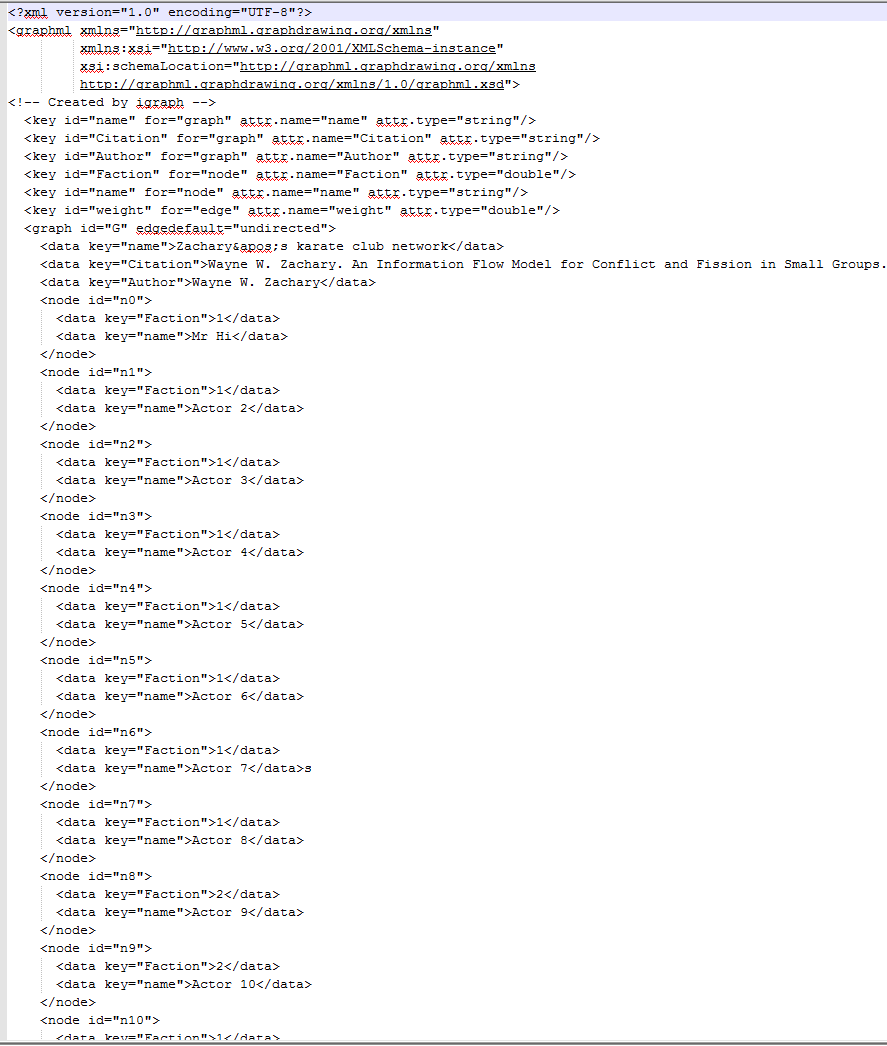
\includegraphics[scale=0.4]{../q3/graphml.png}
\centering
\caption{GraphML data of karate club problem}
\label{}
\end{figure}
\newpage


\subsection{Code Listing}
\subsubsection{convert.py}
\lstinputlisting[breaklines=True,language=Python]{../q3/convert.py}
\newpage


\subsection{Output}
\subsubsection{Without Split}
\begin{figure}[ht]
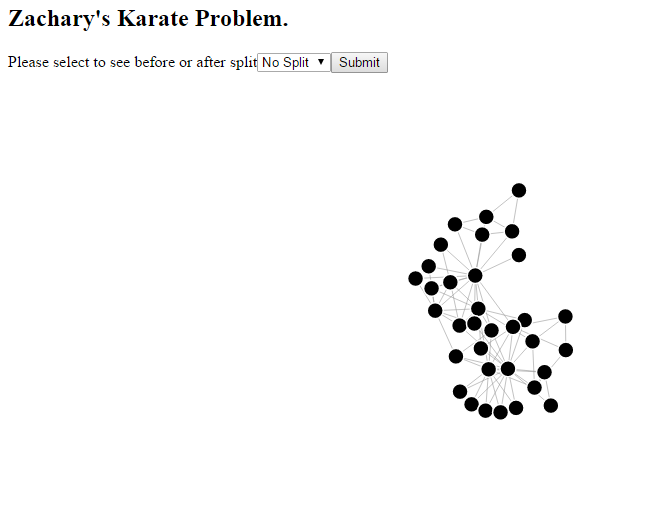
\includegraphics[scale=0.4]{../q3/gr3.png}
\centering
\caption{Karate group without split}
\label{Karate group with split}
\end{figure}


\subsubsection{Karate group with split}
\begin{figure}[ht]
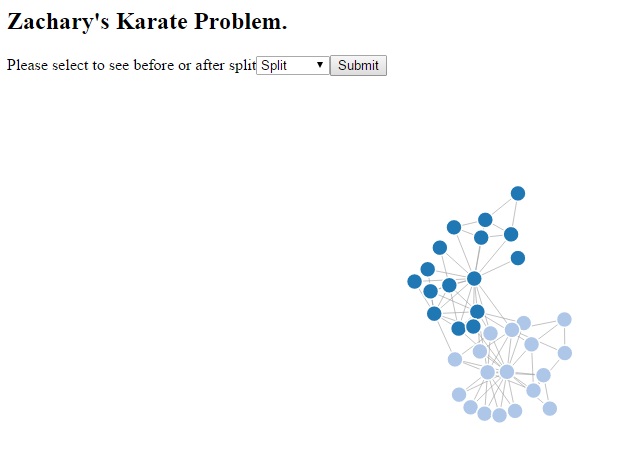
\includegraphics[scale=0.4]{../q3/gr4.png}
\centering
\caption{Karate group with split}
\label{}
\end{figure}
\subsection{URI of graph listed in gist}
\url{http://bl.ocks.org/manojchandrak/raw/50e8ccde5a7e8bc2d5c4/}
\newpage


\addcontentsline{tableofcontents}{section}{References}





\bibliographystyle{plain}
\bibliography{references}
\cite{*}
\end{document}